\section{Results}

We conducted a series of experiments to evaluate the effectiveness of the Kairos system and its components. Our evaluation focuses on two key areas: (1) an ablation study to measure the contribution of the validation and Hebbian learning mechanisms, and (2) a plasticity evaluation to assess the system's ability to learn and adapt over time.

\subsection{Ablation Study}

To quantify the impact of our proposed validation and learning mechanisms, we performed an ablation study comparing the full Kairos system to several ablated configurations. We measured the `trust_score` across a set of 15 questions for each condition. The results are summarized in Table~\ref{tab:ablation}.

\begin{table}[h]
\caption{Ablation Study Results}
\label{tab:ablation}
\centering
\begin{tabular}{lc}
\toprule
\textbf{Ablation Condition} & \textbf{Mean Trust Score} \\
\midrule
Full System & 0.755 \\
No Hebbian Learning & 0.735 \\
No Alignment Validation & 0.793 \\
No Novelty Validation & 0.917 \\
No Logical Validation & 0.706 \\
No Grounding Validation & 0.644 \\
No Validation & 0.000 \\
\bottomrule
\end{tabular}
\end{table}

The results demonstrate the critical importance of the validation layer. When the entire validation layer is disabled (`No Validation`), the `trust_score` drops to 0, as there is no mechanism to assess the quality of the reasoning output. This highlights the necessity of a validation mechanism to prevent the system from blindly trusting the output of the reasoning modules.

The ablation of individual validation nodes also has a significant impact on the `trust_score`. Removing the `GroundingVN` has the most significant impact, reducing the mean `trust_score` to 0.644. This is expected, as the `GroundingVN` is responsible for ensuring that the reasoning is based on facts in the knowledge graph. Removing the `LogicalVN` also has a substantial impact, reducing the `trust_score` to 0.706.

Disabling Hebbian learning (`No Hebbian Learning`) results in a small decrease in the `trust_score` to 0.735. While the immediate impact is modest, the plasticity evaluation in the next section will show the long-term benefits of the Hebbian learning mechanism.

\begin{figure}[h]
    \centering
    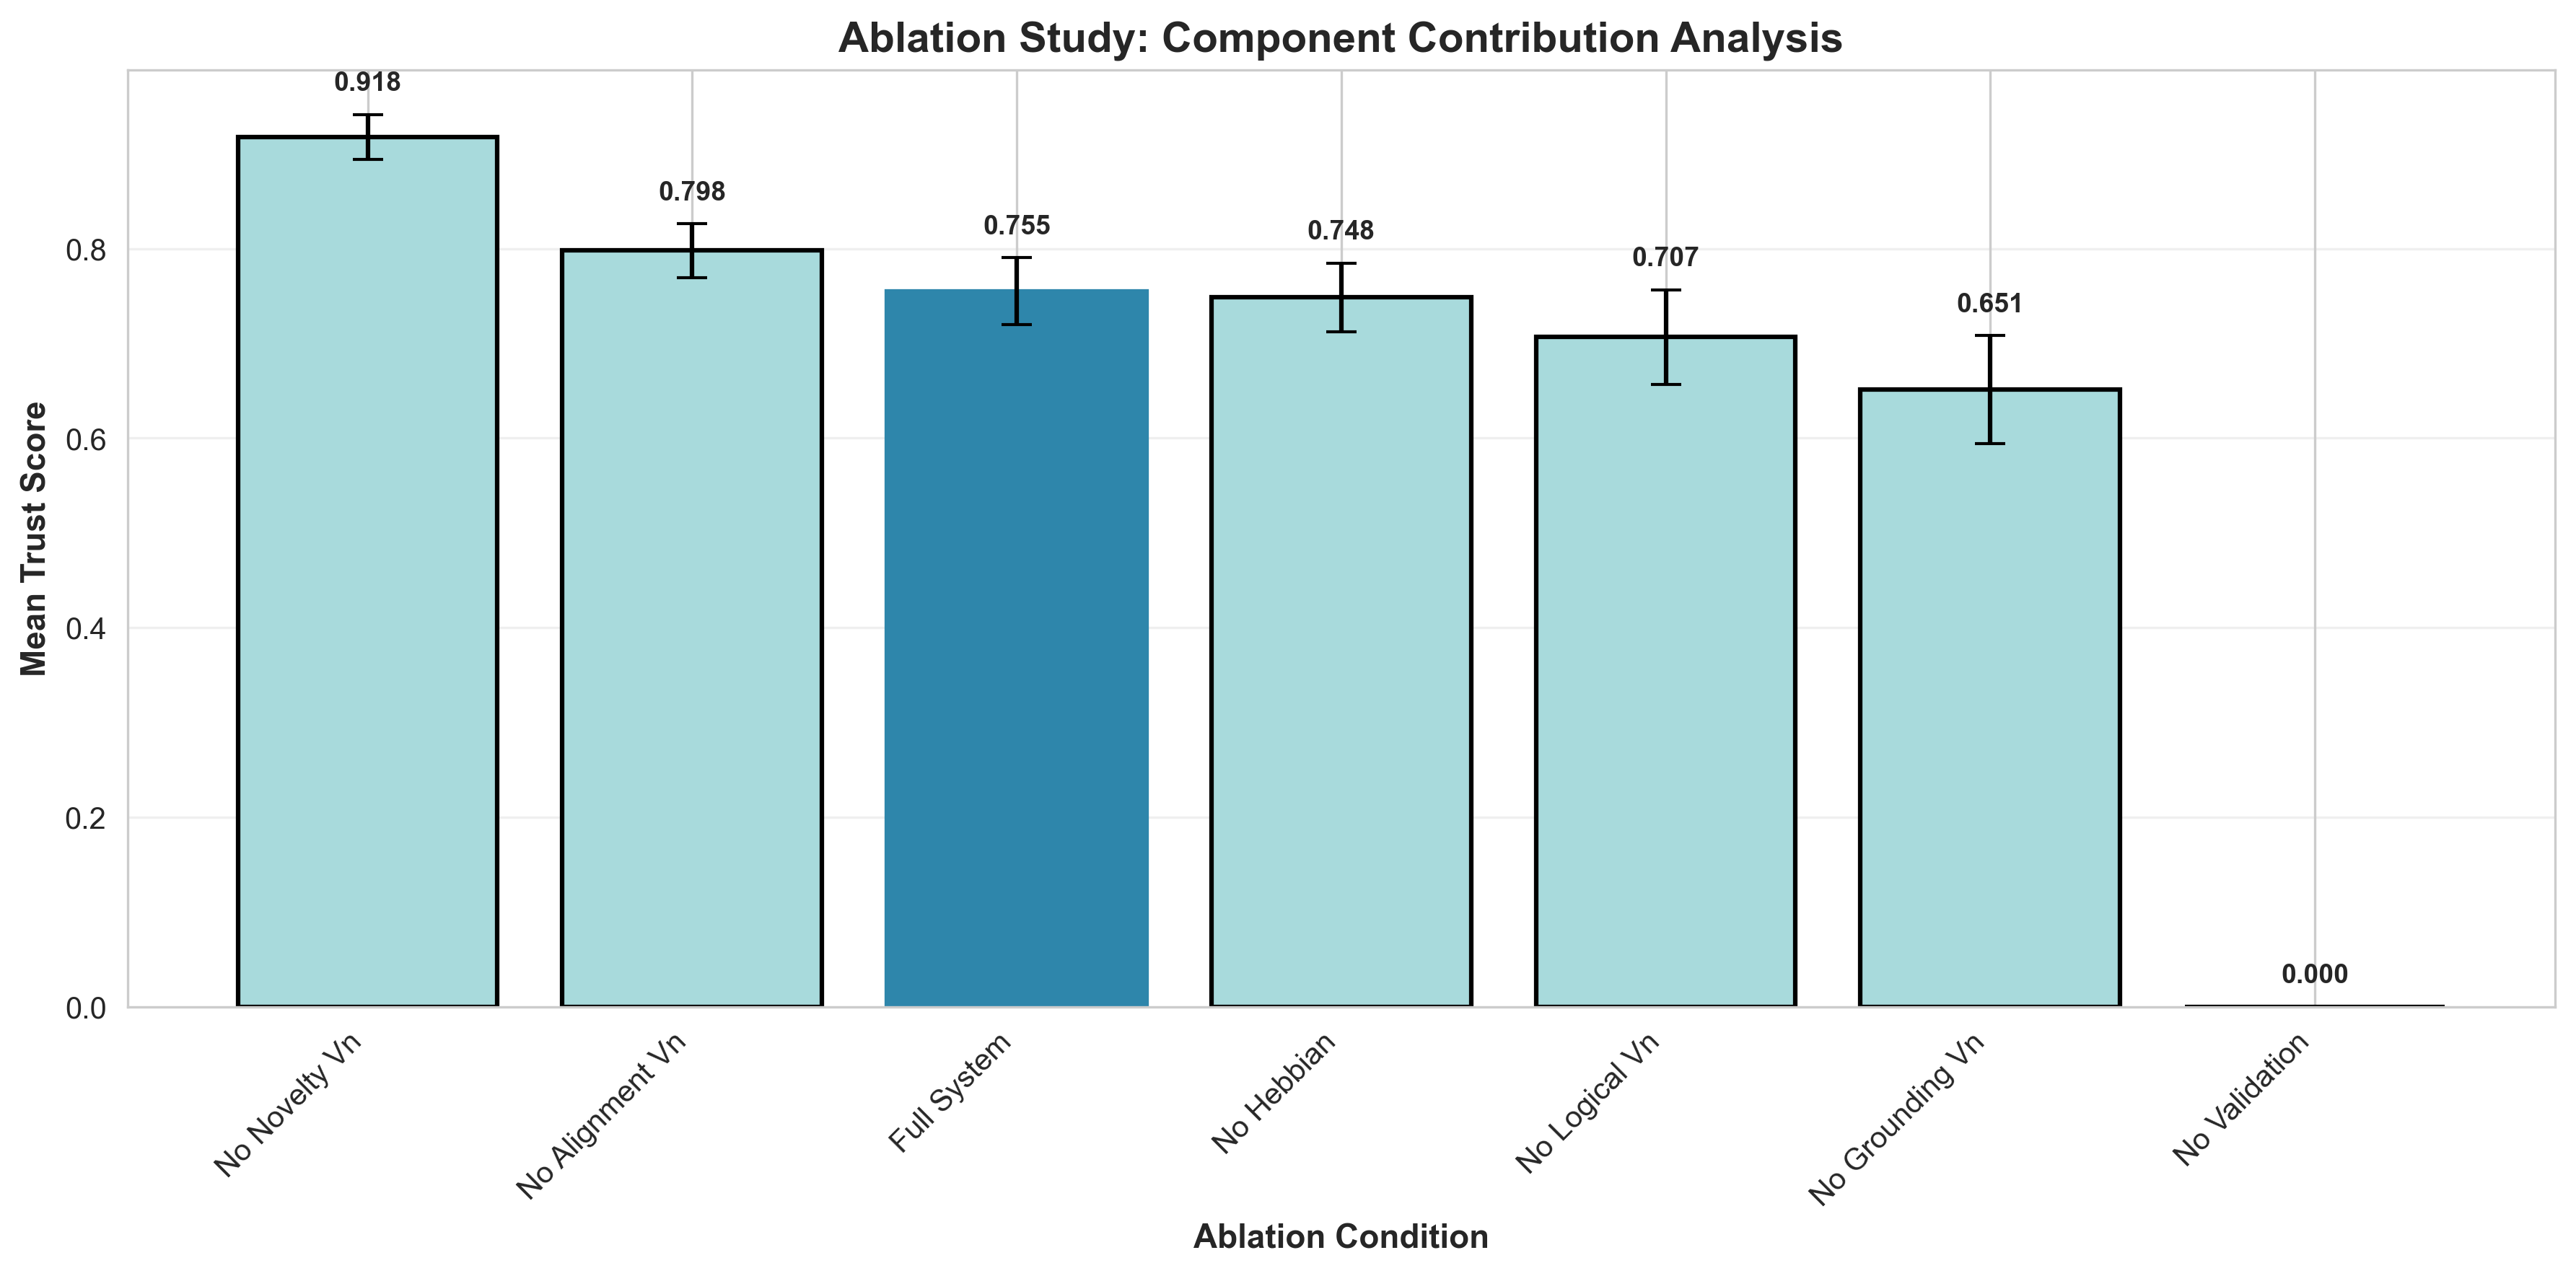
\includegraphics[width=0.8\linewidth]{output/quick_eval_20251027_015729/figures/ablation_comparison.png}
    \caption{Comparison of mean trust scores for each ablation condition.}
    \label{fig:ablation}
\end{figure}

Figure~\ref{fig:ablation} provides a visual comparison of the mean trust scores for each ablation condition. The chart clearly shows the dramatic impact of removing the validation layer and the significant contributions of the grounding and logical validation nodes.

\subsection{Plasticity Evaluation}

To evaluate the effectiveness of the Hebbian learning mechanism, we subjected the system to 5 cycles of reasoning and learning. In each cycle, the system answered a series of questions, and the knowledge graph was updated based on the validation results. We tracked the average strength of the top-k edges in the graph and the number of emergent connections formed.

\begin{figure}[h]
    \centering
    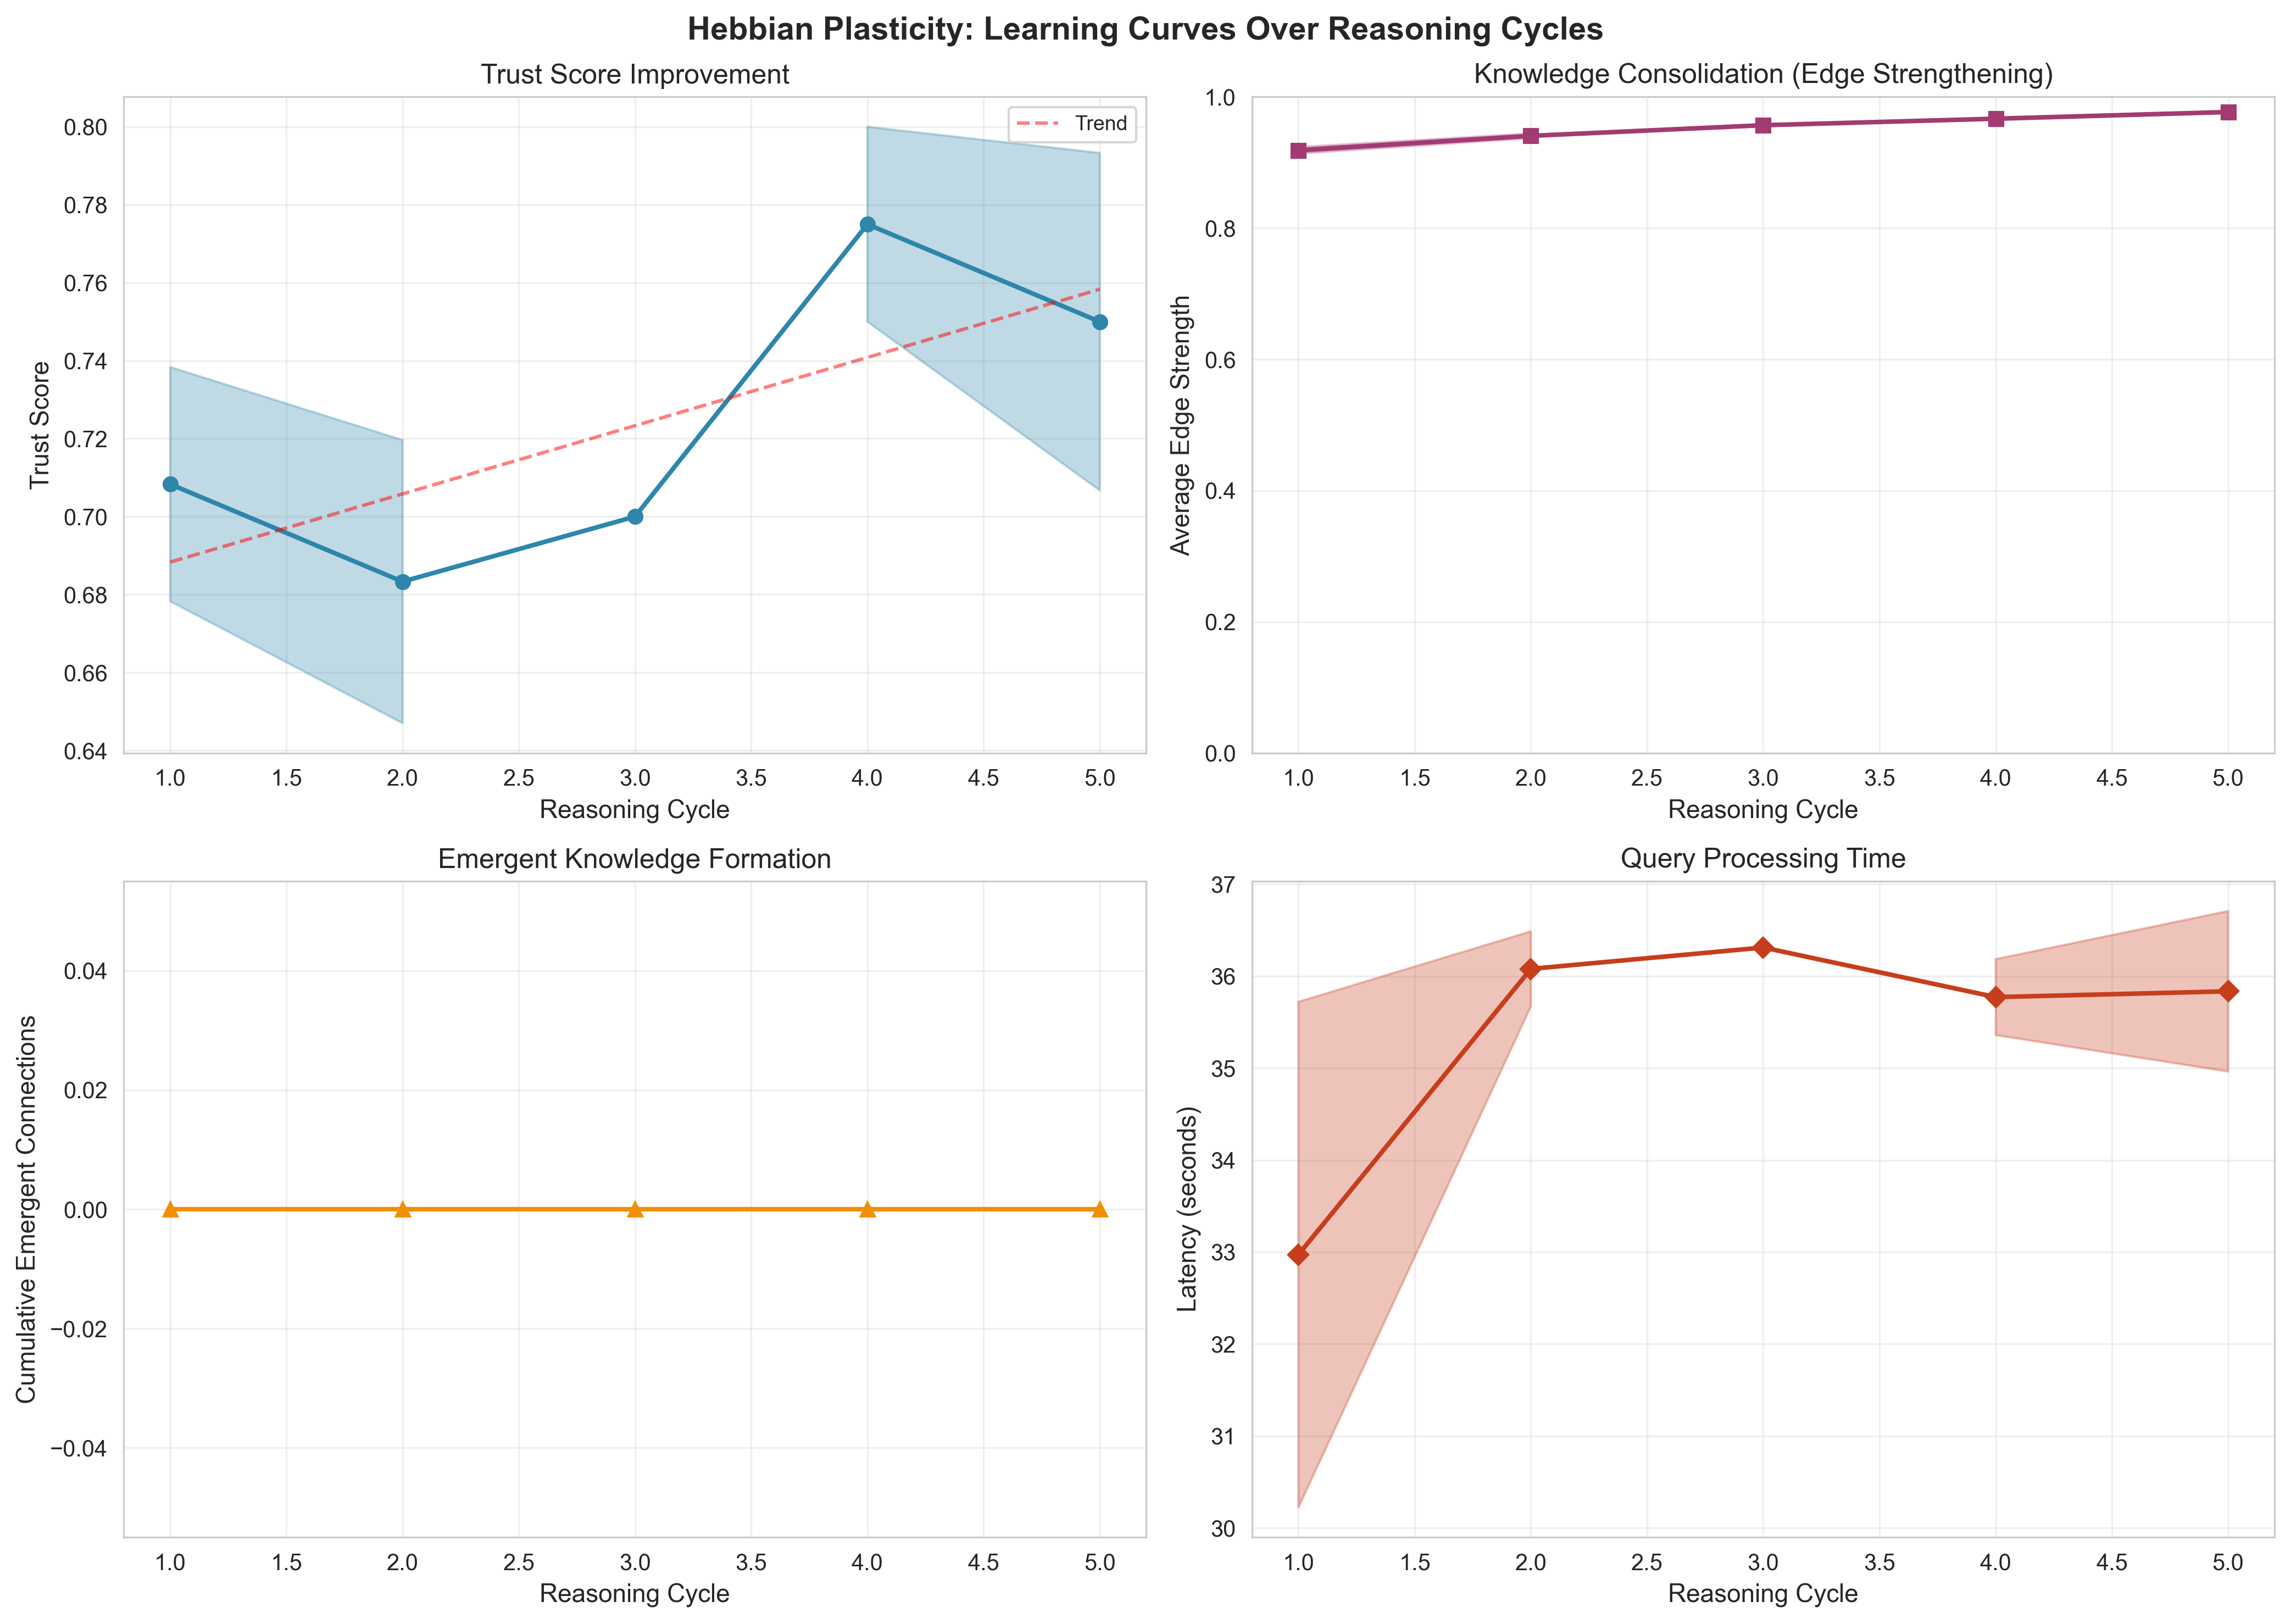
\includegraphics[width=0.8\linewidth]{output/quick_eval_20251027_015729/figures/plasticity_learning_curves.png}
    \caption{Plasticity learning curves showing the evolution of average top-k edge strength over 5 cycles.}
    \label{fig:plasticity_curves}
\end{figure}

As shown in Figure~\ref{fig:plasticity_curves}, the average strength of the top-k edges in the knowledge graph steadily increased over the 5 cycles, from an initial value of 0.9187 to a final value of 0.9770. This demonstrates that the Hebbian learning mechanism is effectively strengthening the connections that are used in successful reasoning paths.

However, we did not observe the formation of any emergent connections during the plasticity evaluation. The number of `emergent_edges_count` remained at 0 throughout the 5 cycles. This is likely due to the `emergence_threshold` of 3 being too high for the limited number of queries in our evaluation. Future work will explore the impact of lower thresholds and more diverse query sets on the formation of emergent connections.

\begin{figure}[h]
    \centering
    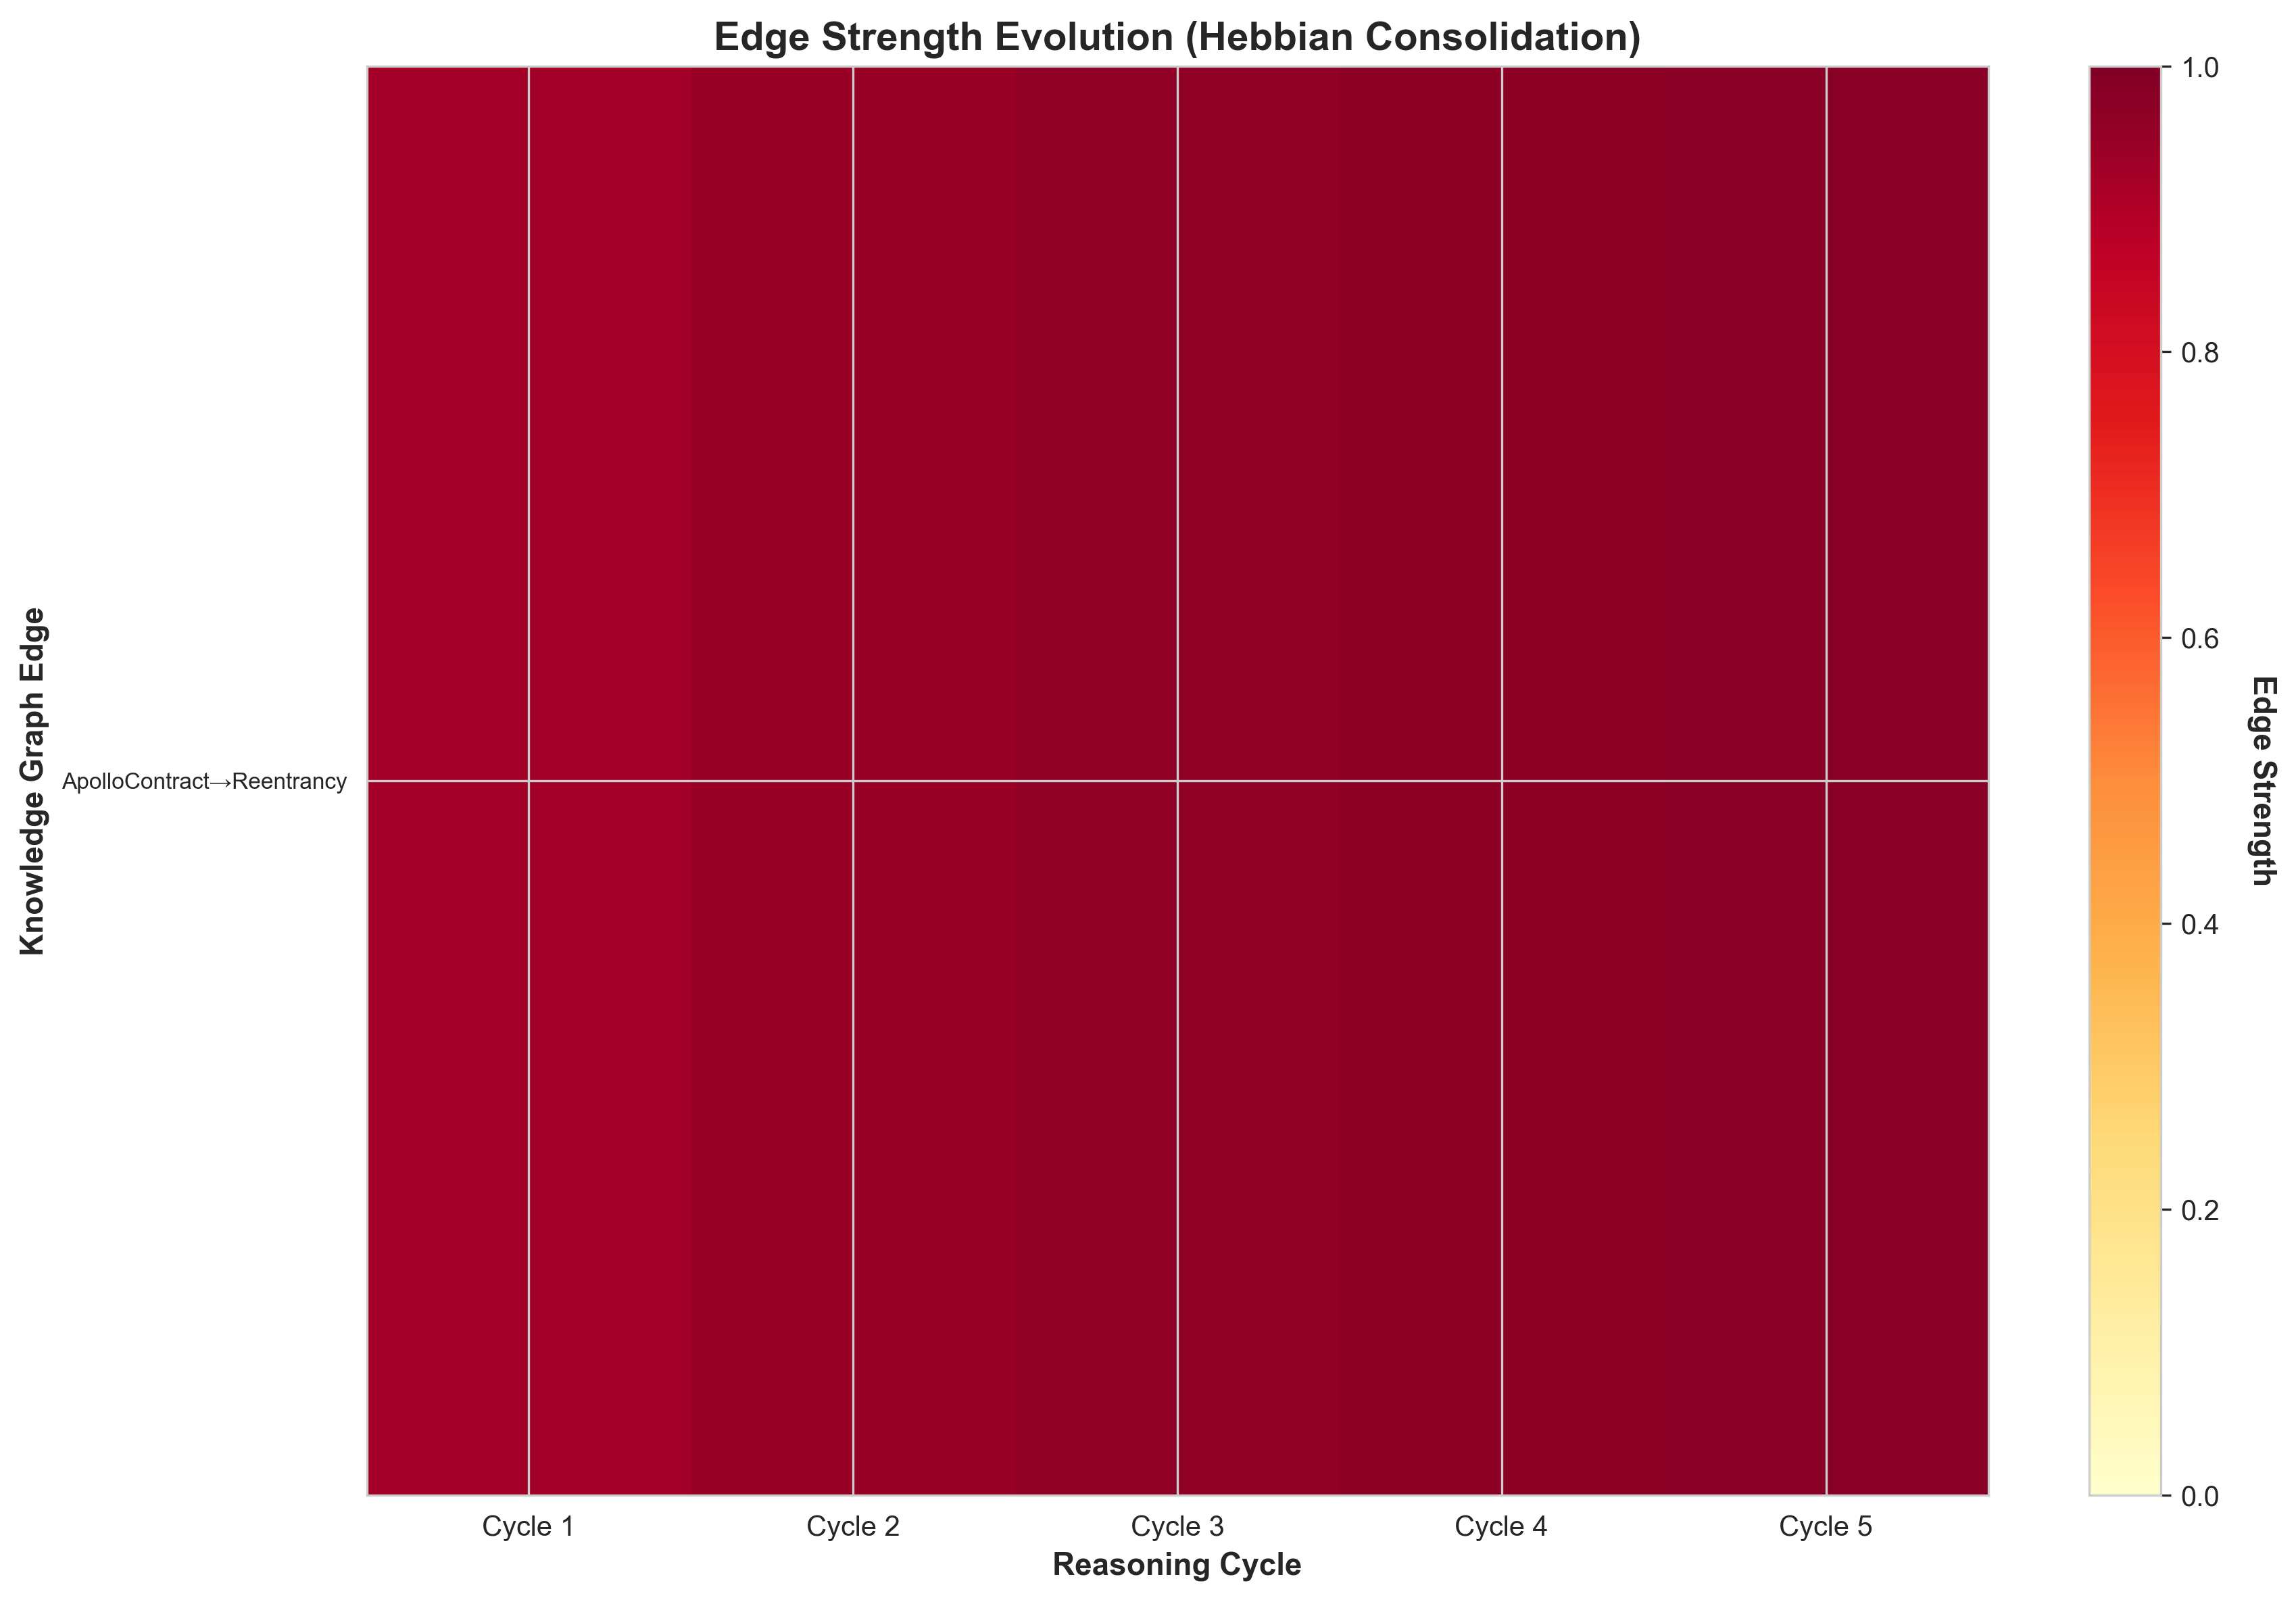
\includegraphics[width=0.8\linewidth]{output/quick_eval_20251027_015729/figures/edge_strength_heatmap.png}
    \caption{Heatmap showing the strength of individual edges in the knowledge graph at the end of the plasticity evaluation.}
    \label{fig:heatmap}
\end{figure}

Figure~\ref{fig:heatmap} shows a heatmap of the edge strengths at the end of the plasticity evaluation. The heatmap clearly shows a small number of very strong edges, which correspond to the most frequently used reasoning paths. This visualization provides further evidence that the Hebbian learning mechanism is effectively identifying and strengthening the most important connections in the knowledge graph.
